\documentclass[11pt]{article}
\usepackage{amsmath,textcomp,amssymb,geometry,graphicx,tikz,cancel}
\usepackage{algpseudocode,algorithm}
\usepackage[T1]{fontenc}
\pagenumbering{gobble}
\usepackage{xcolor}
\usepackage[colorlinks = true,
            linkcolor = blue,
            urlcolor  = blue,
            citecolor = blue,
            anchorcolor = blue]{hyperref}

\newcommand{\MYhref}[3][blue]{\href{#2}{\color{#1}{#3}}}%
\title{BIOE 147 - Detailed Project Description}
\author{Zack Field, Ryan Tsoi}
\date{}
% \noindent\makebox[\linewidth]{\rule{\paperwidth}{9pt}}
\begin{document}
\maketitle


 
%Much of what we have studied in class relies on repressor/activator protein
%and promoter pairs. We have seen that there is a limit to the size of circuit 
%that you can construct, due to the lack of a library of orthogonal proteins.
%While great strides have been made in seeking out new orthogonal repressing/
%activating proteins, it is worth noting that many of the papers that we
%review in lecture still use the same 3 promoter/repressor pairs. 
%It is not a simple task to rationally design our way out of this predicament.
%Since proteins function is dependent upon structure, and the prediction of 
%protein structure is a difficult task (to say the least),
%it would be beneficial to search elsewhere 
%for a class of molecules that can act as a reliable parts family. 
%
%It is already well known that RNA 
%plays a major role in transcriptional, and translational, regulation within 
%the cell  ~\cite{review}. RNA, unlike protein, has well characterized canonical base pairing 
%interactions.  These interactions dominate the formation of secondary structure. 
%Which makes RNA less recalcitrant to rational design than protein ~\cite{howfolds}. Many tools
%have appeared recently that not only quicly and accurately predict RNA secondary structure,
%but also predict tertiary structure (e.g. pseudoknots). Most of the published uses of
%these tools has been focused on thier application to a research topic, rather than
%the implementation of a broad range methodology and workflow for designing 
%RNA-based circuits ~\cite{genetic_switchboard}. An article published last year
%by Keasling's lab states that, with their work, they sought to `establish a foundation for 
%developing computer-aided design platforms' ~\cite{Keasling_Model-Driven}.
%With that in mind, we seek to implement a CAD platform for the compilation of
%biocircuits, that synthesizes the many tools, and techniques that have already
%been detailed, concerning the modeling of riboregulation. The tool itself will
%be similar to simple electrical circuit design tools, and will generate
%algorithmically optimized compositors that can be used to construct a given circuit.
%As an exmaple of the tool's viability, one of the circuits discussed in class, that
%was previously implemented with a repressor-protein/promoter methodology, will be 
%be modeled with a riboregulatory methodology.
%
\section*{Overview}
The goal of this project is create a tool for the rational design of biological 
logic circuits. The interface is a graphical logic circuit tool with drag and
drop functionality of individual gates, switches, and output bulbs. Pictured here
with a repressilator analog and a 4-input AND:

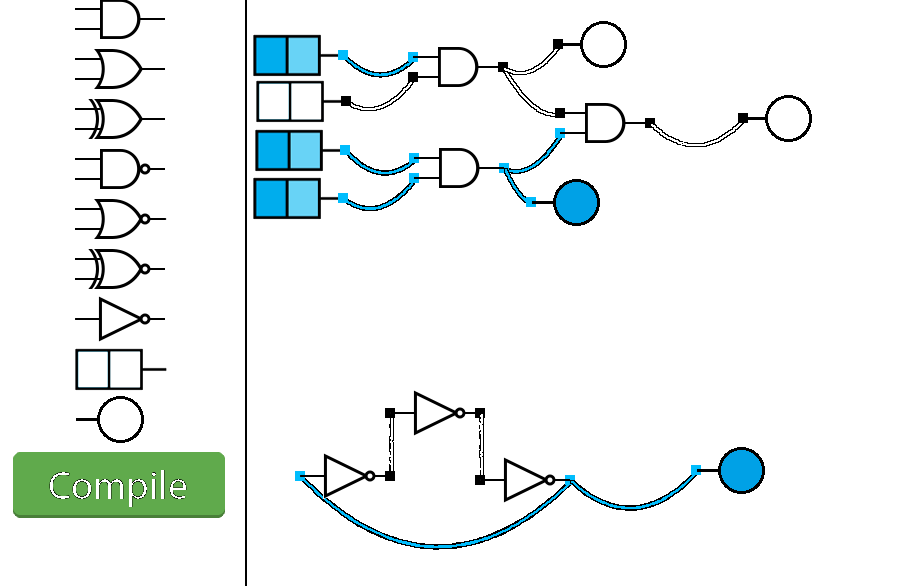
\includegraphics[scale=0.4]{repress_4and.png}

Following the graphical design of a circuit, there is a compilation option
that takes as input the circuit as designed and outputs a set of parts and
compositors that are a good starting point for realizing the circut in vivo.
The details of part and compositor generation are described in the next section.
This type of design flow pulls from design flows that are used in the design of
microelectronic circuits. Analogies can be drawn between the consituents
of semiconductors and biological gates, and these analogies open the door for 
the application of analogous design processes ~\cite{microelectronics}. 

\section*{Compilation}
Since the goal is to generate gates based on user-input, there has to 
be some type of rational, mechanism for generating these gates. 
Of the many types of regulation that occurs
in the cell, riboregulation proves to be the most easily modeled because of the
canonical base pairing interactions that dominate its structure ~\cite{howfolds}.
Because of this, it seemed natural to select riboregulation as the form of regulation
that will be rationally generated by the circuit compiler.
Many models have been created that rely, to varying degrees, on the
quantification of riboregulator libraries ~\cite{arkin_rational}, and on 
thermodynamic free energy calculations ~\cite{Keasling_Model-Driven}. This project does not attempt to devise
a new scheme for predicting RNA-RNA, and RNA-ligand interactions. The chosen scheme
for rational design will be the use of ligand actuated self-cleaving ribozymes as
discussed in Smolke and Win's article ~\cite{smolke_design}. 

The initial inputs to the given circuit will be exogenously added small molecule ligands.
These ligands will bind and modulate the ON/OFF state of a generated ribozyme. The ON 
state is defined as having cleaving ability activated, and conversely, the OFF state is defined
as lacking cleaving ability. The cleaving activity always acts to repress the signal that is downstream of
it, whether that be an siRNA effector or protein coding sequence. The final output signal(s) of the 
circuit  is/are depicted as bulb(s) in the graphical depiction, and they are fluorescent protein(s)
 (xFP, $x\in\{G,R,Y,EB,EC\}$). Now that the initial input signal and final output signal are defined,
the only remaining piece of the circuit is internal signal transduction. A design choice for this tool
is to simply use ribozyme-siRNA pairs. Each of these pairs consists of a ribozyme that is modulated (ON/OFF)
by an effector oligonucleotide, followed by an siRNA. This siRNA acts as the effector oligonucleotide for the 
next ribozyme in the circuit cascade. ~\cite{state_effector} There are many available programs that
assist in secondary structure prediction, but for the purposes of this project 
\MYhref{http://rna.urmc.rochester.edu/rnastructure.html}{RNAstructure v.5.3} 
will be used. This tool has been sucessfully applied by Smolke in the rational design of ribozymes.

The tunable parameters to  be considered are: binding affinities of siRNA/ligand
to a specific ribozyme, and to other non-specific ribozymes, rate of transcription of each 
of the ribozyme-siRNA compositors, degradation rate of each of the ribozyme-siRNA compositors,
activiating/respressing ability of ribozyme when bound/not bound.

Some conceptual constructions of ribozymes upstream of a signal siRNA show how fundamental gates 
can be constructed. The construction of a NOT gate would involve a ribozyme that is ON in 
the presence of an effector oligonucleotide or ligand. An AND gate can be represented
by two ribozymes, adjacent to one another, that are each in the OFF state in the presence of 
two different effector/ligand inputs. Natrually, the two of these gates strung one after another 
will form a functionally complete NAND gate.  

\section*{Additional features}

There are many opportunities to expand on this core design functionality. Given the time
constraint, many of these features will not be realized, but they play a key 
role in describing the power of this type of design tool.
 
\begin{itemize}
\item Logic optimization of graphical logic with \emph{espresso}
\item Graphical parameter optimization that displays transfer curves 
  updated as parameters are changed.
\item Optional use of compositors other than ribozymes and siRNAs.
\item Modeling options during the compilation process (e.g. continuous/stochastic
  model, varying structure prediction algorithms)
\item Automated construction of plasmids, and/or the exporting of compositors to a
  tool like SimVector.
\item Importing logic circuits based on the \emph{espresso} input format 
\item Optional library import for regulators that have been quantified
\end{itemize}
 

\newpage
  
\begin{thebibliography}{9}

\bibitem{review}Chappell, J., Takahashi, M. K., Meyer, S., Loughrey, D., Watters
  , K. E. and Lucks, J.(2013), 
  The centrality of RNA for engineering gene expression. 
  Biotechnology Journal. doi: 10.1002/biot.201300018

\bibitem{howfolds}Ignacio Tinoco Jr, Carlos Bustamante, How RNA folds, 
  Journal of Molecular Biology, Volume 293, Issue 2, 22 October 1999, 
  Pages 271-281, ISSN 0022-2836, http://dx.doi.org/10.1006/jmbi.1999.3001.

\bibitem{automated_design}Guillermo Rodrigo, Thomas E. Landrain, and Alfonso Jaramillo
  De novo automated design of small RNA circuits for engineering synthetic riboregulation in living cells
  PNAS 2012 109 (38) 15271-15276, doi:10.1073/pnas.1203831109

\bibitem{genetic_switchboard}Jarred M. Callura, Charles R. Cantor, and James J. Collins
  Genetic switchboard for synthetic biology applicationsz
  PNAS 2012 109 (15) 5850-5855; published ahead of print March 27, 2012, doi:10.1073/pnas.1203808109

\bibitem{Keasling_Model-Driven}Model-Driven Engineering of RNA Devices to Quantitatively Program Gene Expression
    James M. Carothers, Jonathan A. Goler, Darmawi Juminaga, and Jay D. Keasling
    Science 23 December 2011: 334 (6063), 1716-1719. [DOI:10.1126/science.1212209]

\bibitem{arkin_rational}Mutalik, Vivek K; Qi, Lei; Guimaraes, Joao C; Lucks, Julius B; Arkin, Adam P; ``Rationally designed families of orthogonal RNA regulators of translation'' Nat Chem Biol, 2012/05/

\bibitem{microelectronics}Madec, M.; Lallement, C.; Karstens, K.; Dittman, S.; Gersbacher, M.; Sorg, R.; Wild, M.; Muller, M.; Bourgine, P.; Donzeau, M.; Haiech, J., 
  ``Synthetic biology and microelectronics: A similar design flow,'' Circuits and Systems and TAISA Conference, 2009. NEWCAS-TAISA '09. Joint IEEE North-East Workshop on , vol., no., pp.1,4, June 28 2009-July 1 2009
  doi: 10.1109/NEWCAS.2009.5290444 

\bibitem{smolke_design}Maung Nyan Win and Christina D. Smolke
A modular and extensible RNA-based gene-regulatory platform for engineering cellular function
PNAS 2007 104 (36) 14283-14288; published ahead of print August 20, 2007, doi:10.1073/pnas.0703961104

\bibitem{state_effector}Stephanie Vauleon, Sabine Miller; ``External Regulation of Hairpin
Ribozyme Activity by an'
Oligonucleotide Effector'', ChemBioChem 2003, No. 2-3


\end{thebibliography}

\end{document}
